\section{Video-LDM}
\label{sec:videoldm}

\begin{figure}
    \centering
    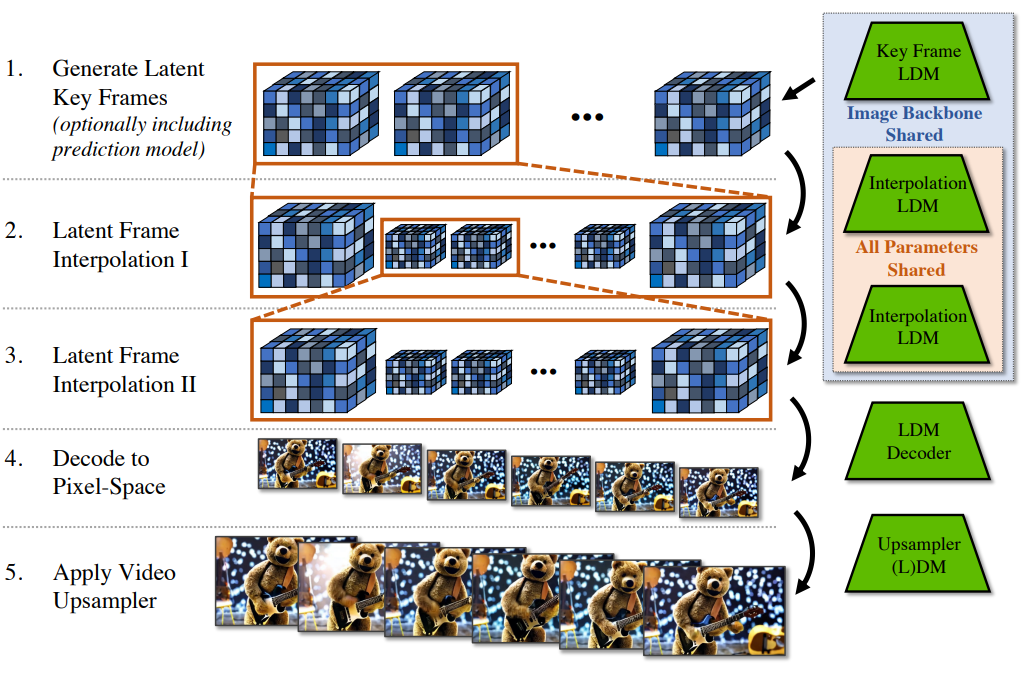
\includegraphics[width=0.7\textwidth]{images/video_ldm/stack.png}
    \caption{Video-LDM stack. (1) The network generates keyframes latents. (2) Between each two keyframes, the network learns to interpolate between (keyframe filling). (3) Between each two frames in the frame filling, they act as new keyframes and the process repeats once more (they use the same interpolation model, same parameters). (4) The latents are decoded to pixel space. (5) Super-resolution model is applied (optionally) to upsample the video resolution.}
\end{figure}

Video-LDM by NVIDIA (2023) \cite{video_ldm} is a text-to-video synthesis model that uses LDM (Latent Diffusion Model, more commonly called Stable Diffusion, section \ref{sec:stable_diffusion}). The main idea of Video-LDM is to first train the model as image generator; and then transform it into a video generator. Its also possible to use pre-trained LDM and then fine-tune it and convert it to a video generator. The model can output in a resolution of up to 1280x2048, which is considered very high resolution in the field of video synthesis.

First, the model is pre-trained with image only datasets; then, temporal layers are added to the LDM that learn to align images in temporally consistent manner; then the model is trained on video datasets and only the temporal layers are learned (the other layers are frozen).

The idea to insert temporal layers into pre-trained generators has been explored by the GAN-based methods MoCoGAN-HD \cite{mocogan_hd} and StyleVideoGAN \cite{style_video_gan} before, but at much smaller scale.

\begin{figure}
    \centering
    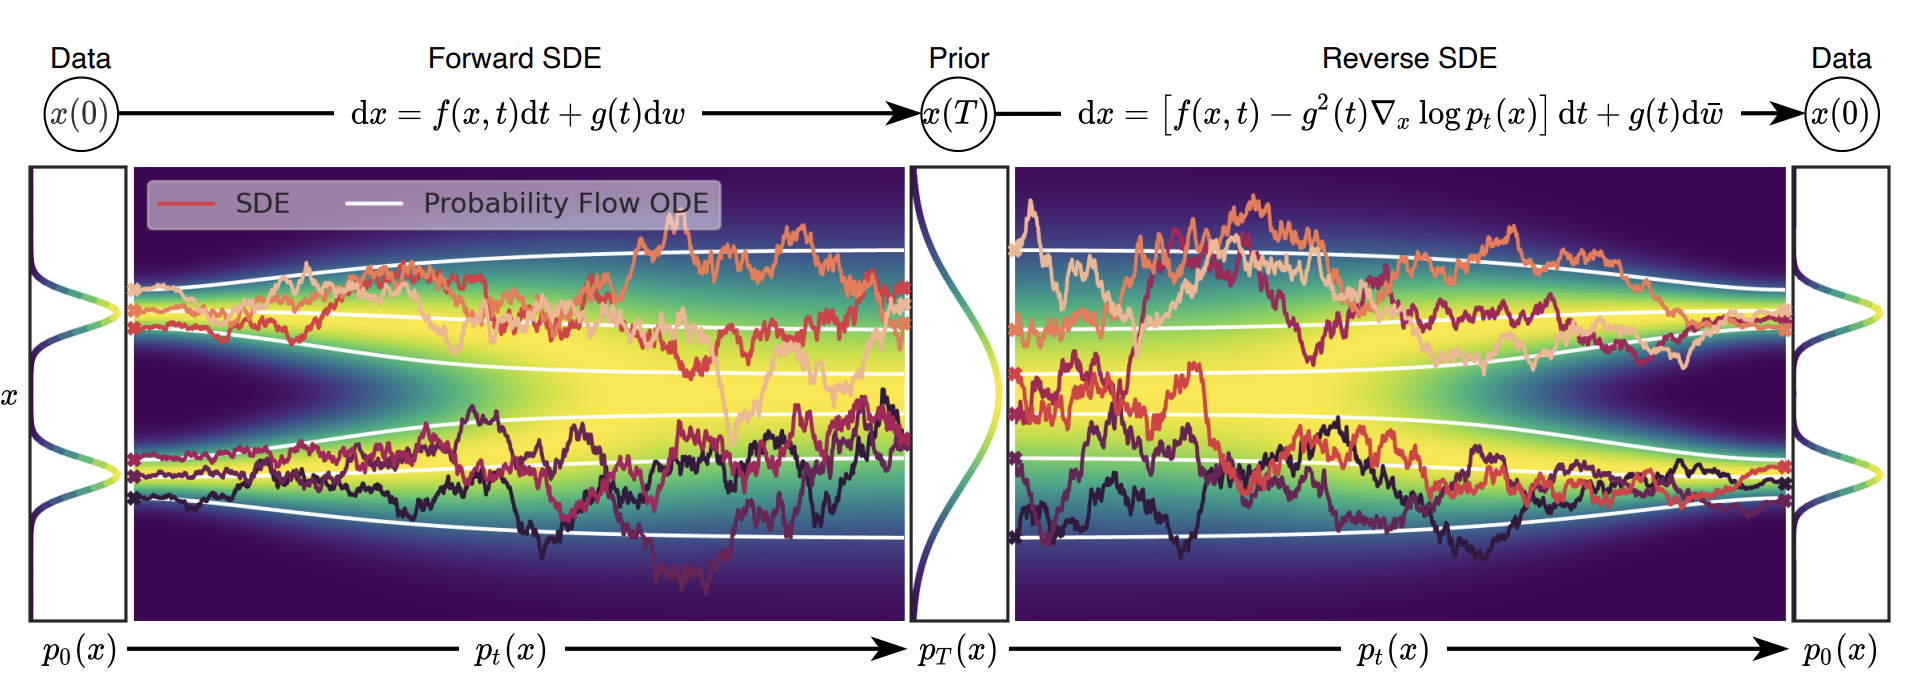
\includegraphics[width=0.8\textwidth]{images/video_ldm/ddpm_sde.png}
    \caption{Generative modeling through stochastic differential equations (SDE) \cite{song2020score}. It shows how data distribution $p(x)$ slowly transforms to prior distribution $p_T(x)$ through forward SDE (we add noise) and then reversed back to generate data with reverse SDE. The colored lines show the SDE paths which represent sample trajectories through the diffusion process. The lines converge at the prior, the noise causes data samples to become progressively less structured, transitioning from a well-defined data distribution to a more chaotic noise-like distribution. The left side shows the probability of the data, the middle shows the probability of the prior (Gaussian distribution), and the right shows we are back to the original data distribution.}
\end{figure}

\begin{figure}
    \centering
    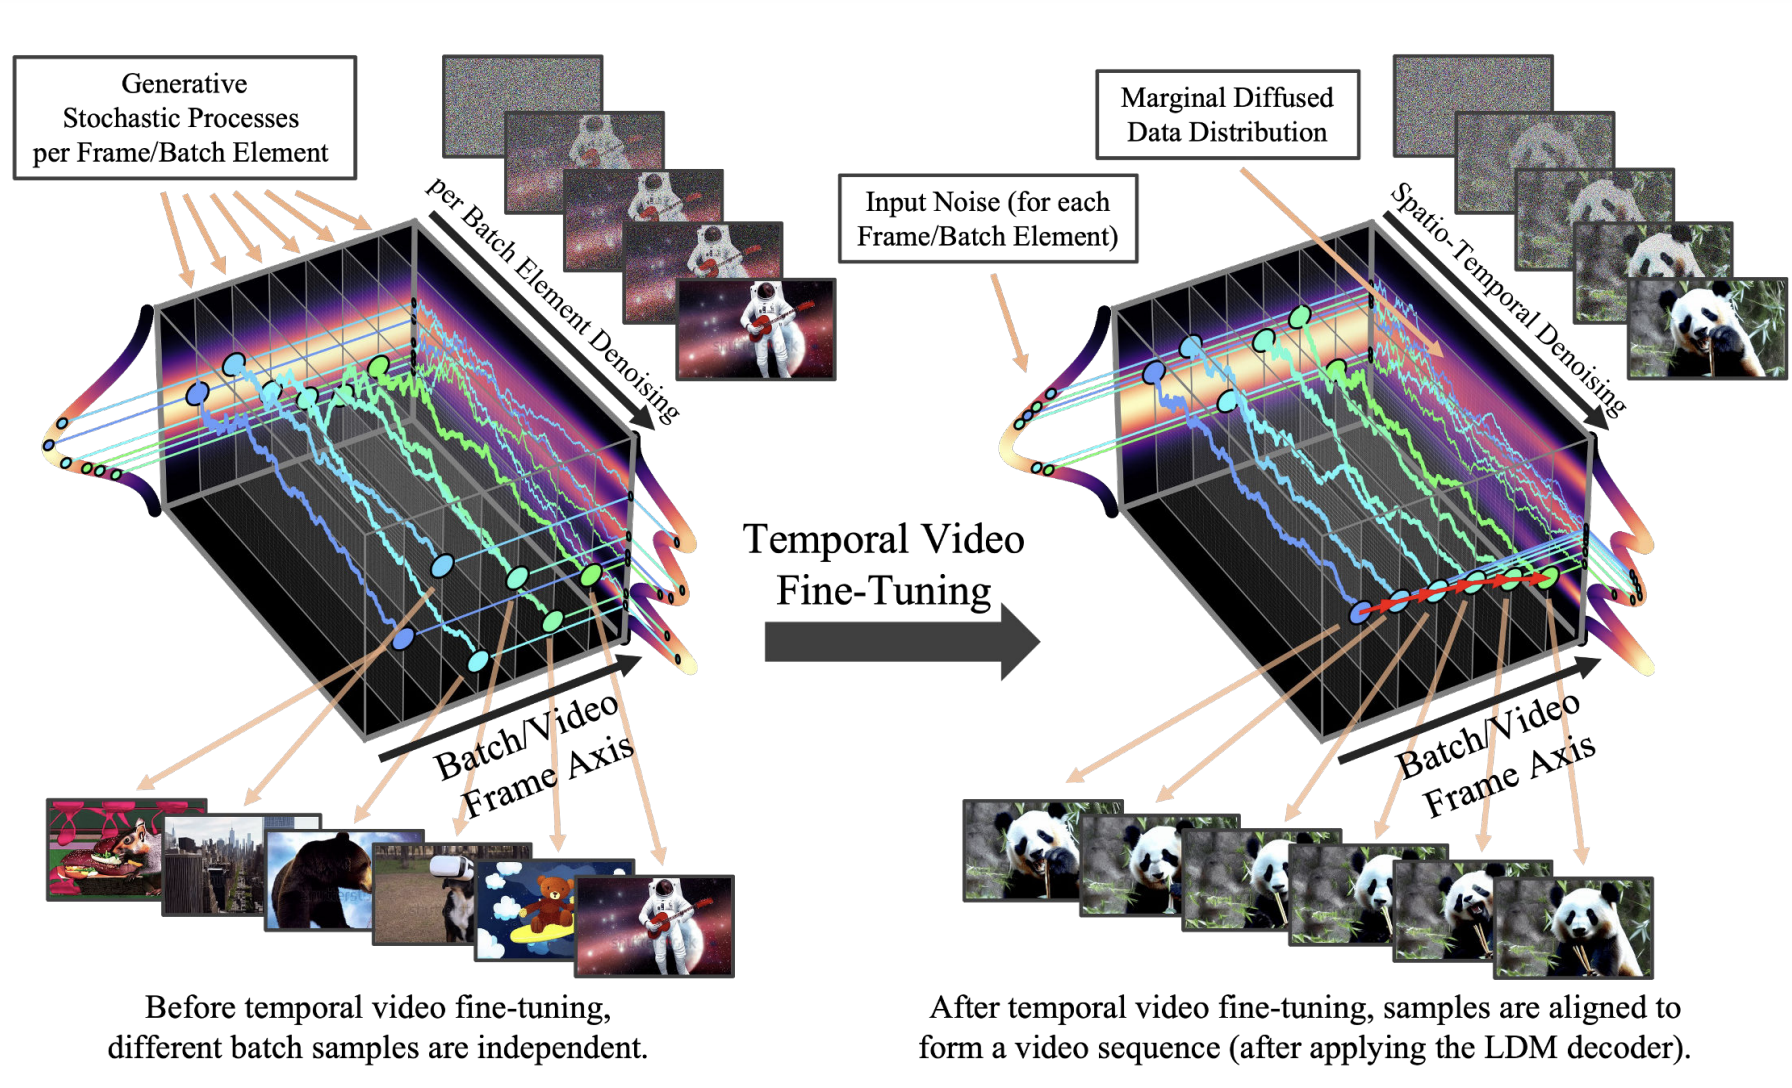
\includegraphics[width=0.8\textwidth]{images/video_ldm/image_to_video_tuning.png}
    \caption{Transforming image LDM (left) to video LDM (right) \cite{video_ldm}. \textit{Per-batch element denoising}: the stochastic denoising process of diffusion. \textit{Batch/Video Frame Axis}: on the left each image generated is not correlated to other images in the batch; on the right each generated image is correlated to the previous image, the model learns to align them and generate temporally consistent video. \textit{Batch/Video Frame Axis}: the red arrows and line shows how one image transitions to the next image, creating the video.}
    \label{fig:video_ldm_image_to_video_tuning}
\end{figure}





\subsection*{Mathematical notations}

The LDMs autoencoder compresses the high-dimensional input data $x \in \mathbb{R}^{T \times 3 \times \hat{H} \times \hat{W}}$ where $x \sim p_{\text{data}}$ is a sequence of $T$ RGB frames with height $\hat{H}$ and width $\hat{W}$ to lower-dimensional latent space $z = \mathcal{E} (x) \in \mathbb{R}^{T \times C \times H \times W}$ (where $C$ is the number of latent channels, and $H, W$ are the spatial latent dimensions) in order to improve computational needs. The model then learns to reconstruct $x$ via decoder $\mathcal{D}$: $\hat{x} = \mathcal{D} (\mathcal{E} (x)) \sim x$.

Let us denote the layers of the LDM (without temporal layers) as spatial layers $l^i_{\theta}$ where $\theta$ are the model's parameters, and $i$ is the layer index. We then denote the addition of temporal layers as $l^i_{\phi}$ to learn to align individual frames in a temporally consistent manner. We denote $f_{\theta, \phi}$ as the full model (with spatial and temporal layers).






\subsection{Architecture}

\begin{figure}
    \centering
    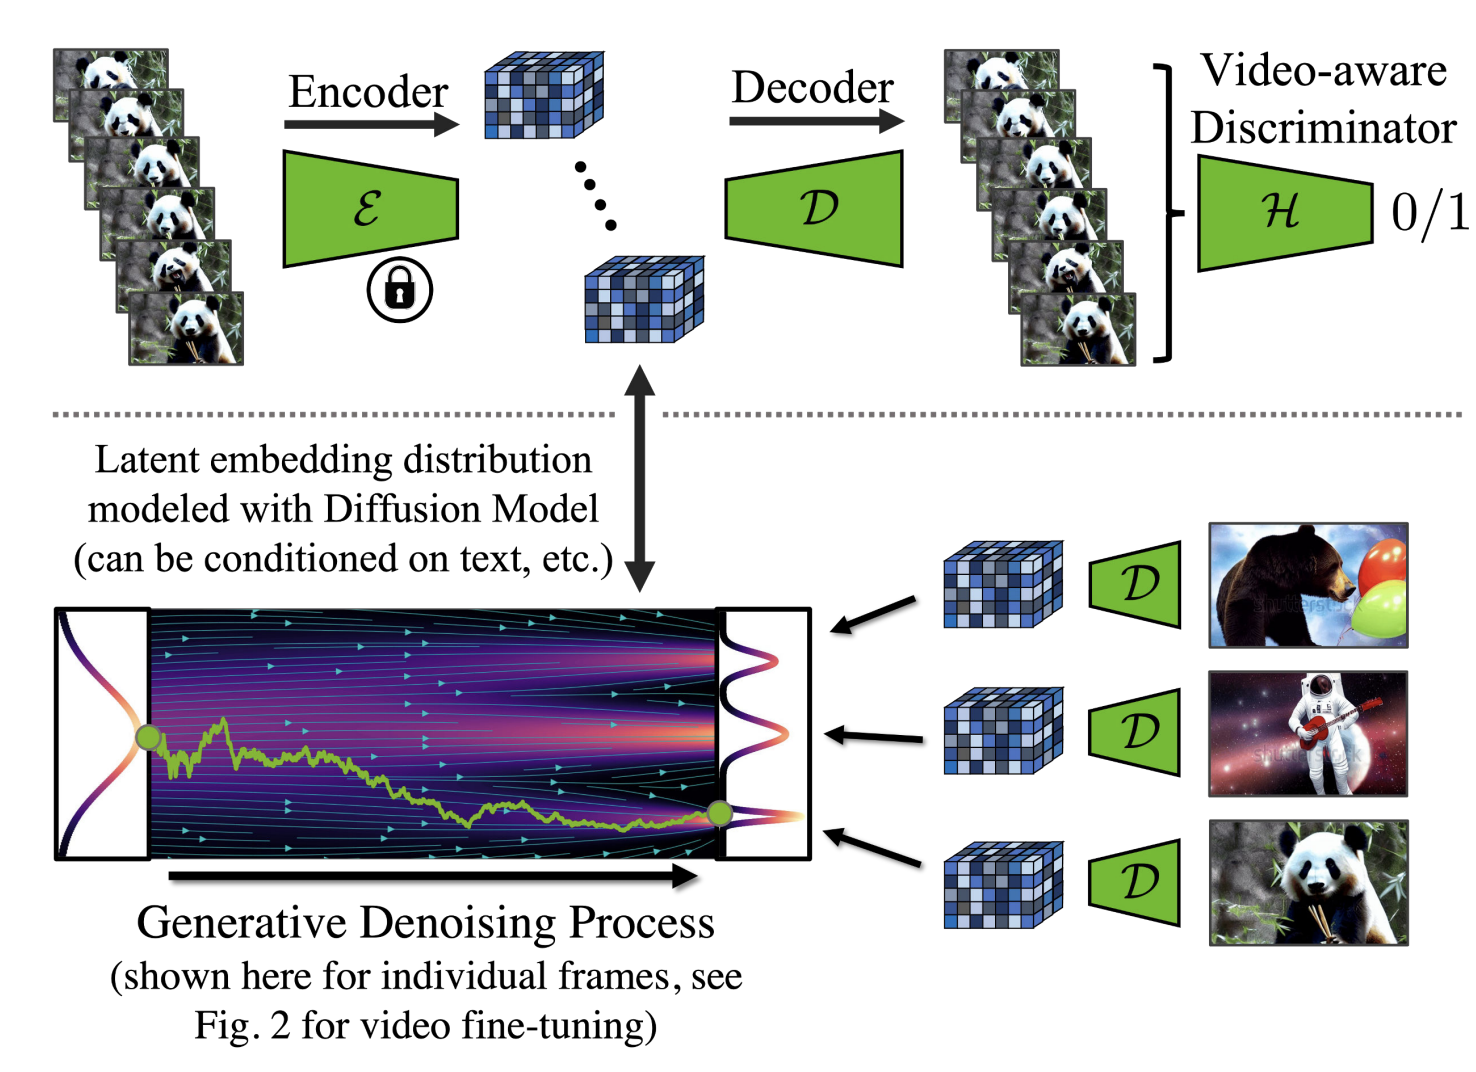
\includegraphics[width=0.6\textwidth]{images/video_ldm/enc_dec_denoise_process.png}
    \caption{Top: frozen encoder compresses video frames into 3D latents and the decoder learns to reconstruct image from the latent (like in autoencoders). The patch-based discriminator $\mathcal{H}$ is used to increase photorealism, the adversarial objective is added to the autoencoder reconstruction score like in PatchGAN (\cite{isola2017image} which tries to classify if $N \times N$ patch is real or fake). \textit{Bottom}: generative denoising process, each embedding corresponds to different image generation in the decoder $\mathcal{D}$.}
\end{figure}

\begin{figure}
    \centering
    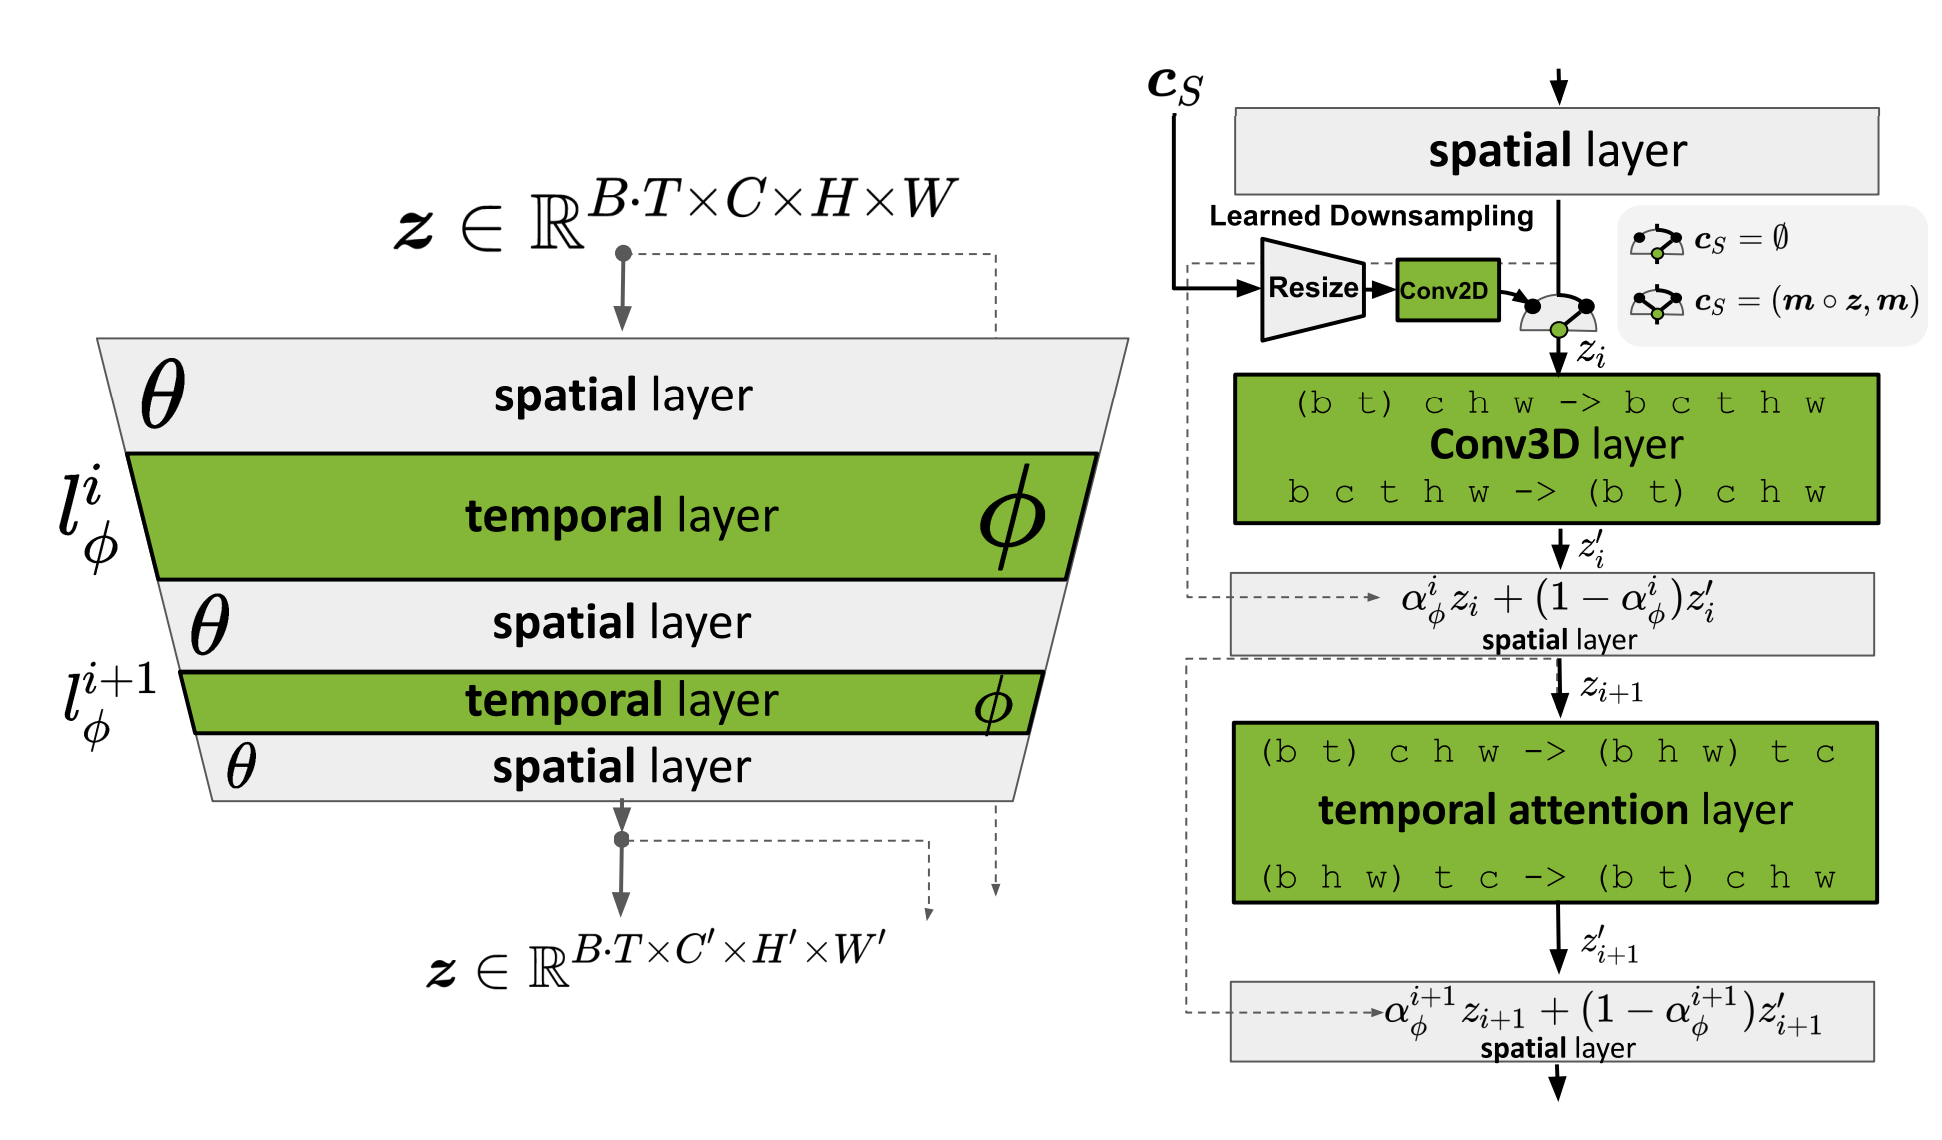
\includegraphics[width=0.6\textwidth]{images/video_ldm/temporal_layers.png}
    \caption{\textit{Left:} The researchers turn pre-trained LDM into video generator by adding temporal layers $l_\phi$ that learn to align images in a temporally consistent manner. The spatial layers $l_\theta$ are frozen and only the temporal layers are learned. \textit{Right:} closer look into spatial, temporal layers of the left side (a single U-Net block). In order to deal with the addition of the temporal dimension, they rearranged the batch dimension in LDM to be mixed with the temporal dimension for the next layer: $(b\ t)\ c\ h\ w \rightarrow b\ t\ c\ h\ w$. The $c_S$ represents a context vector used for conditioning the model.}
    \label{fig:video_ldm_spatial_temporal_mixing_layers}
\end{figure}

The architecture of Video-LDM is similar to Stable Diffusion with the exception of added temporal layers, and the addition of autoencoder for latent encoding/decoding and the discriminator which helps photorealism in the decoder network.

The input of the spatial layers $l_\theta^i$ is of the dimension $b\ c\ h\ w$ whereas the input dimension of temporal layers is of the dimension $b\ t\ c\ h\ w$. This notation is called \texttt{Einops} and is discussed in the Einops paper \cite{einops}. The spatial layers interpret the video as a batch of images by shifting the temporal axis into the batch dimension (the spatial layers treat all $B \cdot T$ encoded video frames in the batch dimension $b$). 

For the 3D convolution (temporal layer), they reshape the input back to video dimensions (they process entire videos in new temporal dimension $t$): 

\[ \underbrace{(b\ t)\ c\ h\ w}_{\text{Output of spatial layer}} \rightarrow \underbrace{b\ c\ t\ h\ w}_{\text{Input to the next Conv3D layer}} \]

After the temporal layers they reshape the input back to fit into the spatial layers like so:

\[ \underbrace{b\ c\ t\ h\ w}_{\text{Output of Conv3D layer}} \rightarrow \underbrace{(b\ t)\ c\ h\ w}_{\text{Input to the next spatial layer}} \]

As for the temporal attention layer (temporal layer), they reshaped the input back to work on the temporal dimension, instead of spatial:

\[ \underbrace{(b\ t)\ c\ h\ w}_{\text{Output of spatial layer}} \rightarrow \underbrace{(b\ h\ w) \ t\ c}_{\text{Input to the next temporal attention layer}} \]

\[ \underbrace{(b\ h\ w) \ t\ c}_{\text{Output of temporal attention layer}} \rightarrow \underbrace{(b\ t)\ c\ h\ w}_{\text{Input to the next spatial layer}} \]

To help us visualize how this reshaping operation works, lets think about 3D cube. The width and height are the spatial width, height of images, and the depth is the temporal dimension (frames of video). Now, lets drop the channels, because its another dimension to think about (each image has 3 channels). Then we can think about temporal operations as a 2D plane slice on the temporal axis. And spatial layers: we can think of them as they work from the width, height dimensions. In both cases, we work in batches, but if we think about batch size of 1 then its easier to understand.

\begin{figure}
    \centering

    \begin{subfigure}{0.3\textwidth}
        \centering
        \scalebox{0.6}{
            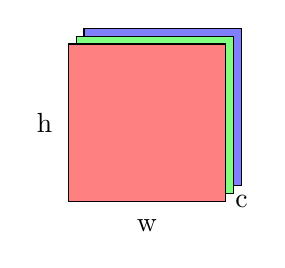
\begin{tikzpicture}
    % Blue channel slice
    \draw[fill=blue!50] (0, 0) rectangle (2, 2);

    % Green channel slice
    \draw[fill=green!50] (-0.1, -0.1) rectangle (1.9, 1.9);
    
    % Red channel slice
    \draw[fill=red!50] (-0.2, -0.2) rectangle (1.8, 1.8);

    \node at (0.8, -0.5) {w};
    \node at (-0.5, 0.8) {h};
    \node at (2, -0.2) {c};
    
\end{tikzpicture}

        }
        \caption{A single frame. The $c\ h\ w$ dimensions.}
    \end{subfigure}

    \begin{subfigure}{0.3\textwidth}
        \centering
        \scalebox{0.6}{
            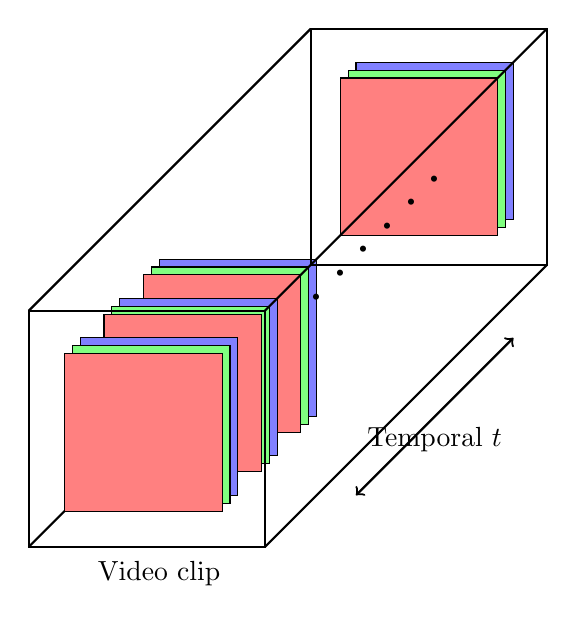
\begin{tikzpicture}
    % 3D Cube - we want to draw some of the cube edges below the frames
    % variables
    \def\cubeWidth{3}
    \def\cubeHeight{3}
    % \def\cubeDepth{8}

    % Cube points
    \coordinate (A) at (0, 0, -5);
    \coordinate (B) at (\cubeWidth, 0, -5);
    \coordinate (C) at (\cubeWidth, \cubeHeight, -5);
    \coordinate (D) at (0, \cubeHeight, -5);
    \coordinate (E) at (-0.5, -0.5, 3);
    \coordinate (F) at (\cubeWidth - 0.5, -0.5, 3);
    \coordinate (G) at (\cubeWidth - 0.5, \cubeHeight - 0.5, 3);
    \coordinate (H) at (-0.5, \cubeHeight - 0.5, 3);

    % Draw cube edges that are below the frames
    \draw[thick] (A) -- (E);

    \def\width{2}
    \def\height{2}
    \def\shift{0.1} % Shift for the green and red channels

    \def\xshift{-0.5}  % Shift in the x direction for duplication
    \def\yshift{-0.5}  % Shift in the y direction for duplication
    \def\lastrectxshift{\xshift * -5} % Last image should be shifted more because of three dots
    \def\lastrectyshift{\yshift * -5} % Last image should be shifted more because of three dots
    \def\dotstartx{2}  % Starting x position for the dots
    \def\dotstarty{1.5}  % Starting y position for the dots
    \def\dotshift{0.3}  % Shift for the dots


    % First rectangle
    \draw[fill=blue!50] (0, 0) rectangle (\width, \height);
    \draw[fill=green!50] (-\shift, -\shift) rectangle (\width-\shift, \height-\shift);
    \draw[fill=red!50] (-2*\shift, -2*\shift) rectangle (\width-2*\shift, \height-2*\shift);

    % Second rectangle
    \draw[fill=blue!50] (\xshift, \yshift) rectangle (\xshift+\width, \yshift+\height);
    \draw[fill=green!50] (\xshift-\shift, \yshift-\shift) rectangle (\xshift+\width-\shift, \yshift+\height-\shift);
    \draw[fill=red!50] (\xshift-2*\shift, \yshift-2*\shift) rectangle (\xshift+\width-2*\shift, \yshift+\height-2*\shift);

    % Third rectangle
    \draw[fill=blue!50] (2*\xshift, 2*\yshift) rectangle (2*\xshift+\width, 2*\yshift+\height);
    \draw[fill=green!50] (2*\xshift-\shift, 2*\yshift-\shift) rectangle (2*\xshift+\width-\shift, 2*\yshift+\height-\shift);
    \draw[fill=red!50] (2*\xshift-2*\shift, 2*\yshift-2*\shift) rectangle (2*\xshift+\width-2*\shift, 2*\yshift+\height-2*\shift);

    % Fourth rectangle
    \draw[fill=blue!50] (\lastrectxshift, \lastrectyshift) rectangle (\lastrectxshift+\width, \lastrectyshift+\height);
    \draw[fill=green!50] (\lastrectxshift-\shift, \lastrectyshift-\shift) rectangle (\lastrectxshift+\width-\shift, \lastrectyshift+\height-\shift);
    \draw[fill=red!50] (\lastrectxshift-2*\shift, \lastrectyshift-2*\shift) rectangle (\lastrectxshift+\width-2*\shift, \lastrectyshift+\height-2*\shift);


    % Dots
    \node at (\dotstartx, \dotstarty) {\huge$\cdot$};
    \node at (\dotstartx + \dotshift, \dotstarty + \dotshift) {\huge$\cdot$};
    \node at (\dotstartx + \dotshift*2, \dotstarty + 2*\dotshift) {\huge$\cdot$};
    \node at (\dotstartx + \dotshift*3, \dotstarty + 3*\dotshift) {\huge$\cdot$};
    \node at (\dotstartx + \dotshift*4, \dotstarty + 4*\dotshift) {\huge$\cdot$};
    \node at (\dotstartx + \dotshift*5, \dotstarty + 5*\dotshift) {\huge$\cdot$};

    % Arrow
    \draw[<->, thick] (2.5, -1) -- (4.5, 1) node[midway, below] {Temporal $t$};







    % Draw the rest of the cube
    \draw[thick] (A) -- (B) -- (C) -- (D) -- cycle;
    \draw[thick] (E) -- (F) -- (G) -- (H) -- cycle;
    \draw[thick] (B) -- (F);
    \draw[thick] (C) -- (G);
    \draw[thick] (D) -- (H);

    % Draw clip text
    \node at (0, -2) {Video clip};

    

\end{tikzpicture}

        }
        \caption{Multiple frames. The $b\ c\ h\ w$ dimensions.}
    \end{subfigure}

    \begin{subfigure}{0.7\textwidth}
        \centering
        \scalebox{0.6}{
            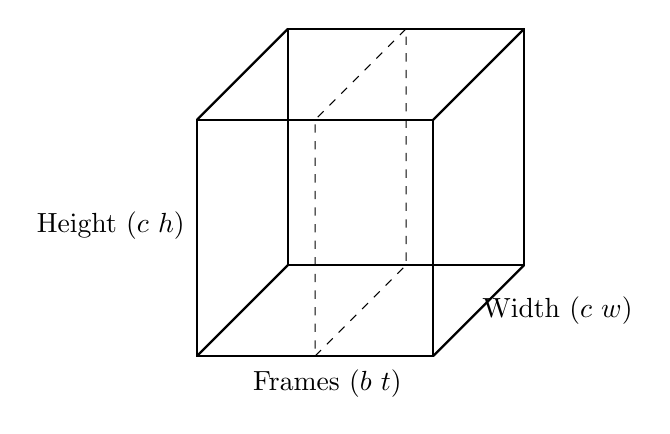
\begin{tikzpicture}
    % Cube points
    \coordinate (A) at (0, 0, 0);
    \coordinate (B) at (3, 0, 0);
    \coordinate (C) at (3, 3, 0);
    \coordinate (D) at (0, 3, 0);
    \coordinate (E) at (0, 0, 3);
    \coordinate (F) at (3, 0, 3);
    \coordinate (G) at (3, 3, 3);
    \coordinate (H) at (0, 3, 3);

    % Draw cube
    \draw[thick] (A) -- (B) -- (C) -- (D) -- cycle;
    \draw[thick] (E) -- (F) -- (G) -- (H) -- cycle;
    \draw[thick] (A) -- (E);
    \draw[thick] (B) -- (F);
    \draw[thick] (C) -- (G);
    \draw[thick] (D) -- (H);

    % Draw slice in middle
    \draw[dashed] (1.5, 0, 3) -- (1.5, 0, 0) -- (1.5, 3, 0) -- (1.5, 3, 3) -- cycle;
    
    % Axes
    \node at (0.5, -1.5, 0) {Frames $(b\ t)$}; 
    \node at (-2.25, 0.5, 0) {Height $(c\ h)$};
    \node at (4.0, 0, 1.5) {Width $(c\ w)$};

    % Add slice label
    % \node at (1.5, 3.5) {$(b\ t)\ c$};
\end{tikzpicture}
        }
        \caption{All of the $b\ t\ c\ h\ w$ dimensions. The temporal dimension is added when applying temporal layers. The slice in the middle shows a single frame of dimension $(b\ t\ c)\ h\ w$, all of the first three dimensions collapse into the channel dimension.}
    \end{subfigure}

    \caption{Representation of video dimensions ($b\ t\ c\ h\ w$ which corresponds to batch, temporal, channel, height, width dimensions in video) to better understand input reshaping in spatial and temporal layers of Video-LDM.}
\end{figure}





\textbf{Mixing factor:} after each temporal layer, the output $z'$ is combined with the output of previous spatial layer output $z$ to form a mixing: 

\[ \underbrace{\alpha_\phi^i z_{i} + (1 - \alpha_\phi^i) z_{i}'}_{\text{Mixing factor}} \] 

where $\alpha_\phi^i \in [0, 1]$ and is a learnable parameter. If we set $\alpha = 1$ for each layer skip the temporal score and we retain the native image generation capability. This mixing operation is similar to Classifier-free Guidance (CFG) (mixing between conditional score and unconditional score).

\textbf{Temporal mixing layers:} two types of temporal mixing layers in use (see figure \ref{fig:video_ldm_spatial_temporal_mixing_layers}) are the \textit{temporal attention} and \textit{Conv3D} layer. The temporal attention layer is similar to the spatial attention layer, but it operates on the temporal dimension.

\textbf{Noise scheduler:} Video-LDM uses the same noise scheduler as the underlying image model. In table 6 of the paper, it shows that in all of their models, they use linear noise scheduler.

\textbf{Training objective:} the training objective is likelihood based, and only the temporal layers are trained. The objective is like the LDM objective (score matching objective of predicted noise in U-Net, basically mean squared error (MSE)):

\[ \arg \min_\phi \mathbb{E}_{x \sim p_{\text{data}}, \tau \sim p_{\tau}, \epsilon \sim \mathcal{N} (0, I)} \left[ \left| \left| y - f_{\theta,\phi} (z_{\tau} ; c, \tau) \right| \right|^2_2 \right] \]

where $\tau$ is the diffusion time step, $y$ is the target noise vector. The target is to minimize the difference between predicted noise and ground truth $y$ over all video frames (with mean squared error).

\textbf{Adding temporal layers to the autoencoder's decoder:} the researchers add temporal layers to the decoder of the autoencoder which they found this step to be critical for achieving good results. The reason is that the autoencoder is trained on images and flickering artifacts are present in the generated videos (because training on images doesn't teach the model temporal dynamics). So the researchers fine-tune the decoder on video data with a \textbf{patch-wise temporal discriminator built from 3D convolutions}. The encoder, however, remains unchanged.

\textbf{Patch-wise temporal discriminator:} The patch-wise temporal discriminator $\mathcal{H}$, which is built from 3D convolutions, is used to fine-tune the autoencoder (decoder only, encoder is frozen) on video data. It takes in video as input, and returns "real" or "fake" prediction on patches of the video clip.


\begin{figure}
    \centering
    \scalebox{0.5}{
        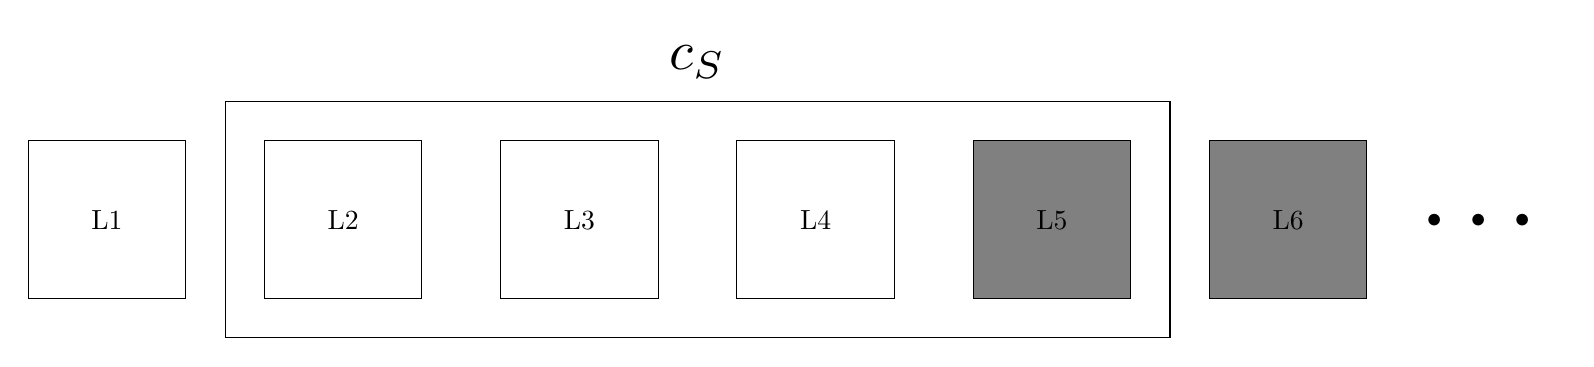
\begin{tikzpicture}
    \draw[fill=white!50] (0, 0) rectangle (2, 2);
    \node[anchor=center] at (1, 1) {L1};

    \draw[fill=white!50] (3, 0) rectangle (5, 2);
    \node[anchor=center] at (4, 1) {L2};

    \draw[fill=white!50] (6, 0) rectangle (8, 2);
    \node[anchor=center] at (7, 1) {L3};

    \draw[fill=white!50] (9, 0) rectangle (11, 2);
    \node[anchor=center] at (10, 1) {L4};

    \draw[fill=black!50] (12, 0) rectangle (14, 2);
    \node[anchor=center] at (13, 1) {L5};

    \draw[fill=black!50] (15, 0) rectangle (17, 2);
    \node[anchor=center] at (16, 1) {L6};

    % c_S
    \node[anchor=center, scale=2] at (8.5,3) {$c_S$};

    % Context guidance box
    \draw[] (2.5, -0.5) rectangle (14.5, 2.5);

    % 3 Dots
    \node [scale=4] at (18,1) {\rotatebox{90}{$\vdots$}};
\end{tikzpicture}
    }
    \caption{Keyframe model learns to predict the next latent frame $z$ by context guidance (conditioned on previous frames).}
\end{figure}

\begin{figure}
    \centering
    \scalebox{0.5}{
        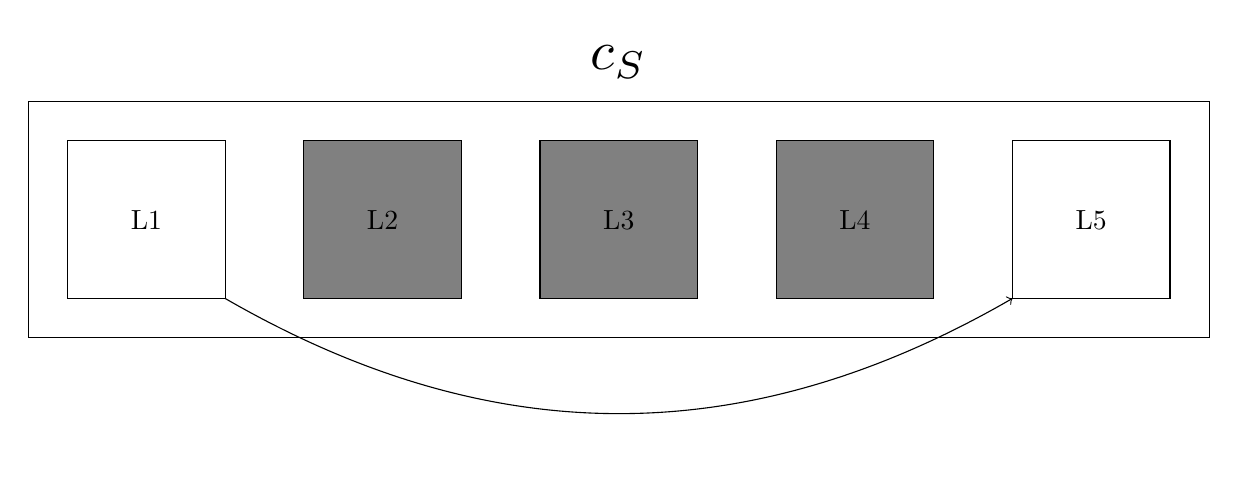
\begin{tikzpicture}
    \draw[fill=white!50] (0, 0) rectangle (2, 2);
    \node[anchor=center] at (1, 1) {L1};

    \draw[fill=black!50] (3, 0) rectangle (5, 2);
    \node[anchor=center] at (4, 1) {L2};

    \draw[fill=black!50] (6, 0) rectangle (8, 2);
    \node[anchor=center] at (7, 1) {L3};

    \draw[fill=black!50] (9, 0) rectangle (11, 2);
    \node[anchor=center] at (10, 1) {L4};

    \draw[fill=white!50] (12, 0) rectangle (14, 2);
    \node[anchor=center] at (13, 1) {L5};

    \draw[->] (2, 0) to[bend right] (12, 0);

    \node[anchor=center, scale=2] at (7,3) {$c_S$};
    \draw[] (-0.5, -0.5) rectangle (14.5, 2.5);
\end{tikzpicture}
    }
    \caption{Interpolation model learns to fill masked latents $m \circ z$ (L2, L3, L4) in between two keyframes latents (L1, L5) with context guidance.}
\end{figure}

\textbf{Context guidance \& Masking:} the model can be conditioned on context information, and is denoted with $c_S$ in figure \ref{fig:video_ldm_spatial_temporal_mixing_layers}. For long video synthesis, the model is conditioned on the initial set of $S$ context frames, which are the frames at the beginning of the clip. A temporal binary mask is applied to the frames that the model must predict, so the model knows which frames it must predict and which is the context guidance. The latent vector generated by the encoder is concatenated with the binary mask, forming the context guidance $c_S$.

\textbf{Temporal binary mask:} generating latents and turning them into video (temporal autoregressive is frame-by-frame prediction) is efficient, but it reaches its limits when generating long duration videos. In order to adapt to longer duration videos, the researchers trained models as \textit{prediction models} where for each two keyframes, interpolate between them (divide and conquer). By using \textbf{binary masks} $m_S$ (0 or 1) it indicates the model which frames and the context ($m = 1$) and which frames are to be predicted $m = 0$. The frames are multiplied by the mask and the model learns to predict the missing frames.

\textbf{Higher frame rate:} to achieve high frame rate (high temporal resolution), they predict three interpolated frames between each two keyframes; they call this $T \rightarrow 4T$ \textbf{interpolation model}. Its possible to achieve higher frame rates; its also possible to train $4T \rightarrow 16T$ interpolation model. They use the same interpolation model twice in order to further increase the frame rate.

\textbf{LDM Decoder: } after the interpolation models, the latents are then decoded to pixel space using the LDM decoder.

\textbf{Upsampler (L)DM: } to increase the spatial resolution of generated frames, they used a super-resolution (SR) model, which increases the output resolution by $4 \times $. They take inspiration from cascaded DMs \cite{cascaded_diffusion_models}, which we already discussed in Imagen (the SR3 model \cite{sr3}). In their experiments they used \textbf{pixel-space DM}, whereas for text-to-video models they used \textbf{LDM upsampler}. This step is optional, since its just for increasing the resolution of the generated video. However, since upsampling video frames independenly would result in poor temporal consistency, they made the SR model video-aware by adding temporal layers and mixing spatial and temporal layers, in similar manner as discussed before.

\textbf{Number of parameters: } the Video-LDM model (except for the CLIP text encoder) consists of 3.1 billion parameters (autoencoder and diffusion models), and only 2.2 billion of these parameters are actually trained:

\begin{itemize}
    \item 84 million parameters in the autoencoder
    \item 865 million parameters in the image backbone LDM, not including CLIP text encoder
    \item 655 million parameters in temporal layers
    \item 354 million parameters in the text encoder (OpenCLIP-ViT/H)
    \item 1.5 million parameters in the interpolation latent diffusion model
\end{itemize}

Compared to Imagen (11.6 billion parameters) and CogVideo (9 billion parameters), Video-LDM is much smaller yet produced high quality videos, because it works in latent space.

\textbf{DDIM Sampling:} in appendix F of the paper they write that they use the sampler from denoising diffusion implicit models (DDIM) \cite{ddim} (section \ref{subsec:ddim_sampler}), where the stochastically $\eta$ is varied, as well as the guidance scale.

\textbf{CLIP text encoder: } the text encoder (for text-to-video model conditioning) is CLIP \cite{openai_clip} based which is used to generate text embeddings, as we discussed before (section \ref{subsec:clip}).










\subsection{Experiments}

\begin{figure}
    \centering
    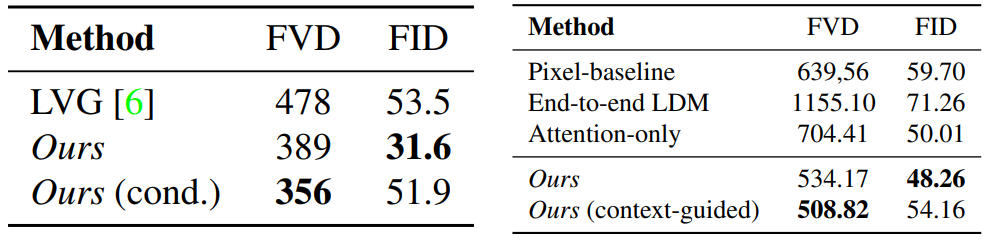
\includegraphics[width=0.5\textwidth]{images/video_ldm/videoldm_vs_lvg_on_rds.png}
    \caption{\textit{Left}: Comparison of Video-LDM and Long Video GAN (LVG) on RDS dataset. \texttt{Cond.} means the model was conditioned on day/night and crowdedness. Side note: adding conditional information reduces FID and FVD. \textit{Right}: FVD and FID evaluations on different diffusion architectures (pixel-space diffusion model, end-to-end LDM that was not pre-trained on images [which is why the results are bad], and attention-only temporal model). Their model uses 3D temporal convolutions which is better than the attention-only diffusion model.}
    \label{fig:video_ldm_vs_lvg_on_rds}
\end{figure}

\begin{figure}
    \centering
    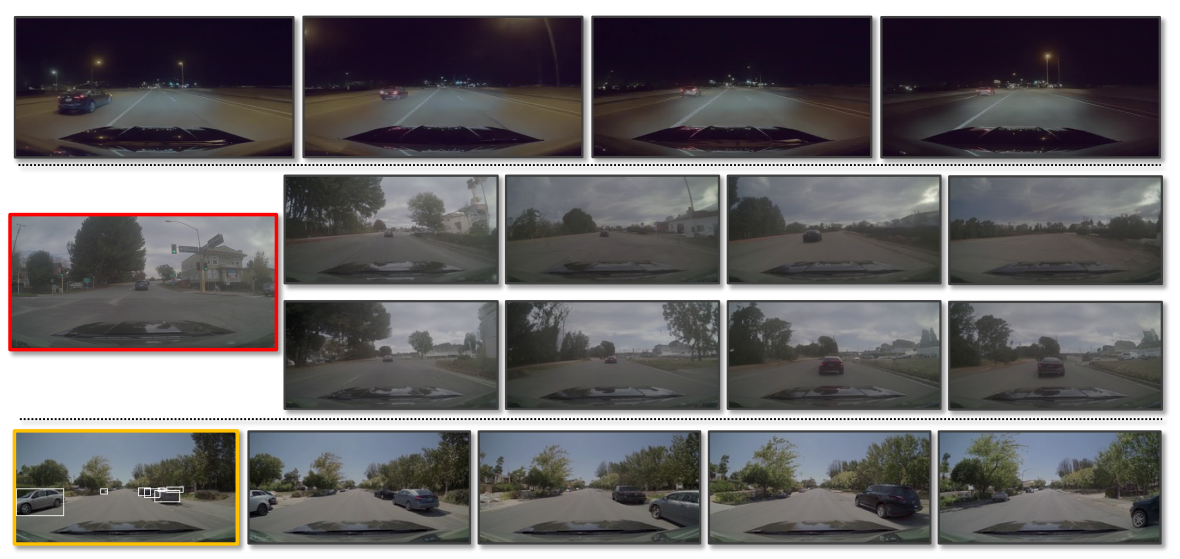
\includegraphics[width=0.7\textwidth]{images/video_ldm/rds.png}
    \caption{Real driving videos (RDS) generation samples. \textit{Top}: night videos. \textit{Middle:} the left red frame is the condition input, while the right is two different generated samples (given a frame, the model can generate the next frames). \textit{Bottom}: they trained a seperate bounding-box conditioned LDM for image synthesis only (the RDS dataset has some bounding-box clips), which generates initial frame (in yellow), and then Video-LDM completes the video generation based on this frame.}
\end{figure}

\begin{figure}
    \centering
    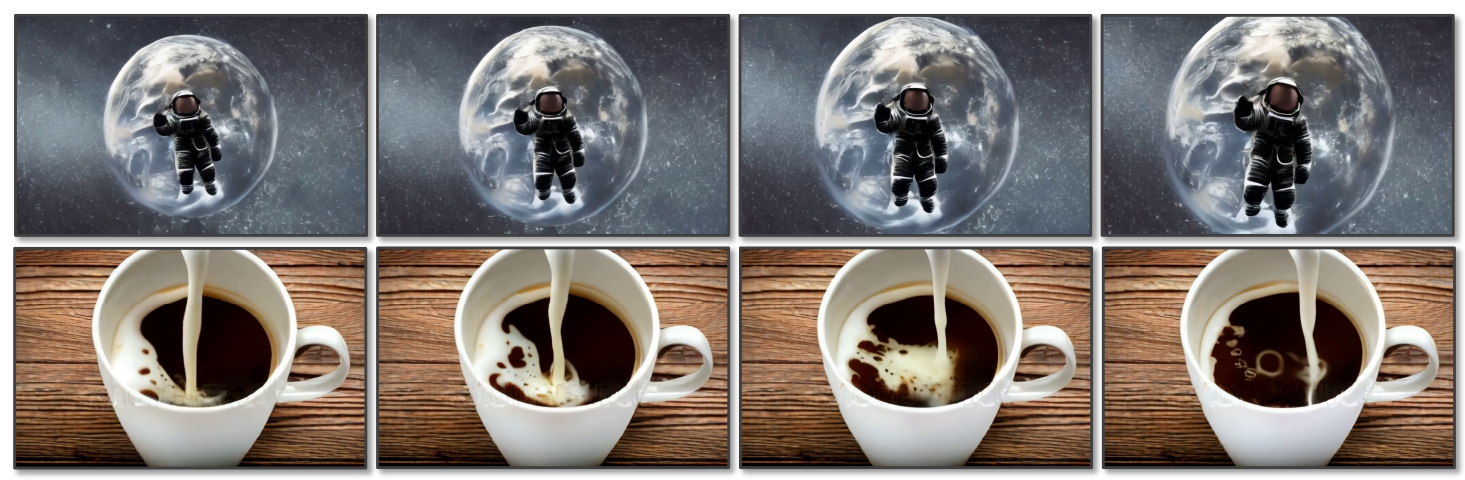
\includegraphics[width=0.7\textwidth]{images/video_ldm/webvid_samples.png}
    \caption{Generated samples at $1280\times 2048$ resolution trained on WebVid-10M dataset. Prompts: "An astronaut flying in space, 4k, high resolution" and "Milk dripping into a cup of coffee, high definition, 4k".}
\end{figure}

\begin{figure}
    \centering

    \begin{subfigure}{0.45\textwidth}
        \centering
        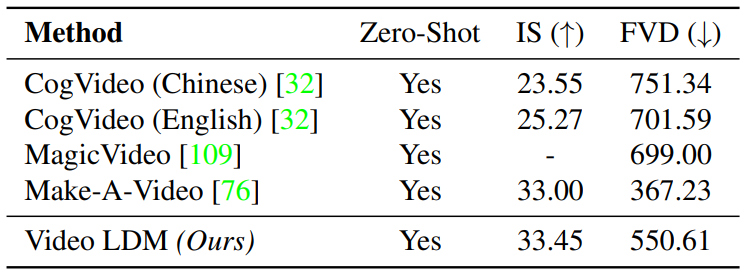
\includegraphics[width=0.8\linewidth]{images/video_ldm/ucf.png}
        \caption{UCF-101 dataset. Video-LDM achieves the best inception score.}
    \end{subfigure}

    \begin{subfigure}{0.45\textwidth}
        \centering
        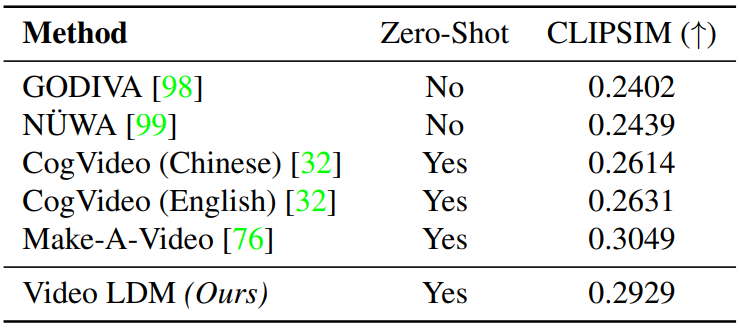
\includegraphics[width=0.8\linewidth]{images/video_ldm/msr_vtt.png}
        \caption{MSR-VTT dataset. Video-LDM almost achieves the best CLIP-SIM score.}
    \end{subfigure}

    \caption{Zero-shot text-to-video synthesis on UCF-101 and MSR-VTT datasets. Video-LDM is compared to other state-of-the-art models in zero-shot setting.}
\end{figure}




The researchers used the following datasets:

\begin{itemize}
    \item In-house dataset of real driving videos (RDS). The dataset consists of 683,060 videos up to 8 seconds long at 512x1024 resolution, and frame rate up to 30 fps. The dataset has day and night driving videos, annotation of number of vehicles ("crowdedness") and some of them even have bounding boxes of cars. They conditioned on day/night labels and crowdedness and randomly dropped these labels during training to allow for classifier-free guidance and unconditional synthesis. The previous state-of-the-art model in terms of long-term high-resolution video synthesis was Long Video GAN (LVG) \cite{brooks2022generating} is compared to Video-LDM on the same dataset in figure \ref{fig:video_ldm_vs_lvg_on_rds}.
    \item WebVid-10M dataset \cite{bain2021frozen} that contains 10.7 million video-caption pairs with total of 52K hours. For this experiment, they turned a publicly available Stable Diffusion model into a text-to-video synthesis model by adding temporal alignment layers. First, they fine-tuned the spatial layers on frames from the dataset and only then insert the temporal layers. Then, they freeze the spatial layers and train only the temporal layers on WebVid-10M videos with the addition the caption (text) of the dataset. In similar manner, they fine-tuned the Stable Diffusion upsampler which can upscale by $4\times$ the frames and generate videos at $1280\times 2048$ resolution (the dataset clips resolution is $320\times 512$). The samples are 113 frames, which translates either to 4.7 second @ 24 fps or 3.8 seconds @ 30 fps.
    \item Mountain bike dataset \cite{brooks2022generating} which was introduced by Long Video GAN paper consists of 1,202 video clips of varying, but at least 5 seconds length at 30 fps. Details and samples are in the Video-LDM paper.
\end{itemize}

\textbf{Evaluation metrics: } they used FID to evaluate quality of individual frames. They also used FVD and human evaluation on video clips compared to LVG: it was a user study, 100 videos @ 4 seconds, given pair of videos (one from Video-LDM and one from LVG), and participants select the most favorable. For text-to-video model, they evaluated CLIP similarity (CLIP-SIM), and also inception score. They used the ViT-B/32 \cite{openai_clip} model by OpenAI to compute the CLIP score.

In their experiments they \textbf{successfully generated very long temporally coherent high-resolution driving videos of multiple minutes (up to 5 minutes long!)}.

\textbf{Video synthesis on RDS dataset: } for video synthesis on RDS dataset, they first generate a single frame using the image LDM, then they run the prediction model on a \textbf{single frame}, to generate a sequence of key frames. Then, they call the prediction model again, but condition on \textbf{two frames}. Next they optionally perform two steps of the interpolation model which increases the FPS from 1.875 to 7.5 and from 7.5 to 30 fps. And then, optionally they run the patch-wise upsampler which is run over portions of 8 video frames (the upsampler is also temporally aligned).
